% Uncomment for handout
%\def\HANDOUT{}


\ifdefined\HANDOUT
\documentclass[handout]{beamer}
\usepackage{pgfpages}
\pgfpagesuselayout{4 on 1}[letterpaper,landscape,border shrink=5mm]
\else
\documentclass{beamer}
\fi

\mode<presentation>
{
  \usetheme{Warsaw}
  \definecolor{sered}{rgb}{0.78, 0.06, 0.18}
  \definecolor{richblack}{rgb}{0.0, 0.0, 0.0}
  \setbeamercolor{structure}{fg=sered,bg=richblack}
  %\setbeamercovered{transparent}
}


\usepackage[english]{babel}
\usepackage[latin1]{inputenc}
\usepackage{times}
\usepackage[T1]{fontenc}
\usepackage{tikz}
\usepackage{graphicx}
\usepackage[export]{adjustbox}
\usepackage{fancyvrb}
\usepackage{amsmath}
\usepackage{amssymb}
\usepackage{esvect}

\makeatletter
\newcommand{\imagesource}[1]{{\centering\hfill\break\hbox{\scriptsize Image Source:\thinspace{\tiny\itshape #1}}\par}}
\newcommand{\image}[3][\@nil]{%
        \def\tmp{#1}%
        \begin{center}
        \ifx\tmp\@nnil
            \includegraphics[max height = 0.55\textheight, max width = \textwidth]{images/#2}
        \else
            \includegraphics[max height = 0.50\textheight, max width = \textwidth]{images/#2}
            \linebreak
            #1
        \fi
        \linebreak
        {\tiny Image Source:\thinspace{\tiny #3}}
        \end{center}
}

\newenvironment{code}{%
 \VerbatimEnvironment
 \begin{adjustbox}{max width=\textwidth, max height=0.7\textheight}
 \begin{BVerbatim}
  }{
  \end{BVerbatim}
 \end{adjustbox}
}

\title{Cyber Camp: Introduction to Programming}


\author{Dr. Bob Lowe}

\institute[Southeast Missouri State University] % (optional, but mostly needed)
{
  Department of Computer Science\\
  Southeast Missouri State University
}

\date[]{}
\subject{}

\pgfdeclareimage[height=1.0cm]{university-logo}{images/semo-logo}
\logo{\pgfuseimage{university-logo}}



\AtBeginSection[]
{
  \begin{frame}<beamer>{Outline}
    \tableofcontents[currentsection]
  \end{frame}
}


\begin{document}

\begin{frame}
  \titlepage
\end{frame}

\begin{frame}{Outline}
  \tableofcontents
\end{frame}


% Structuring a talk is a difficult task and the following structure
% may not be suitable. Here are some rules that apply for this
% solution: 

% - Exactly two or three sections (other than the summary).
% - At *most* three subsections per section.
% - Talk about 30s to 2min per frame. So there should be between about
%   15 and 30 frames, all told.

% - A conference audience is likely to know very little of what you
%   are going to talk about. So *simplify*!
% - In a 20min talk, getting the main ideas across is hard
%   enough. Leave out details, even if it means being less precise than
%   you think necessary.
% - If you omit details that are vital to the proof/implementation,
%   just say so once. Everybody will be happy with that.

\section{Introduction}

\begin{frame}{What is Programming?}
    \begin{center}
        {\huge What is programming?}
    \end{center}
\end{frame}

\begin{frame}{Micro:Bit}
    \begin{columns}
    \column{0.5\textwidth}
    \begin{itemize}
        \item 62 MHz ARM Cortex-M4 32-bit Processor
        \item 512KB ROM
        \item 128KB RAM
        \item Programming Languages: Python, C++, JavaScript, Scratch
    \end{itemize}
    \column{0.5\textwidth}
    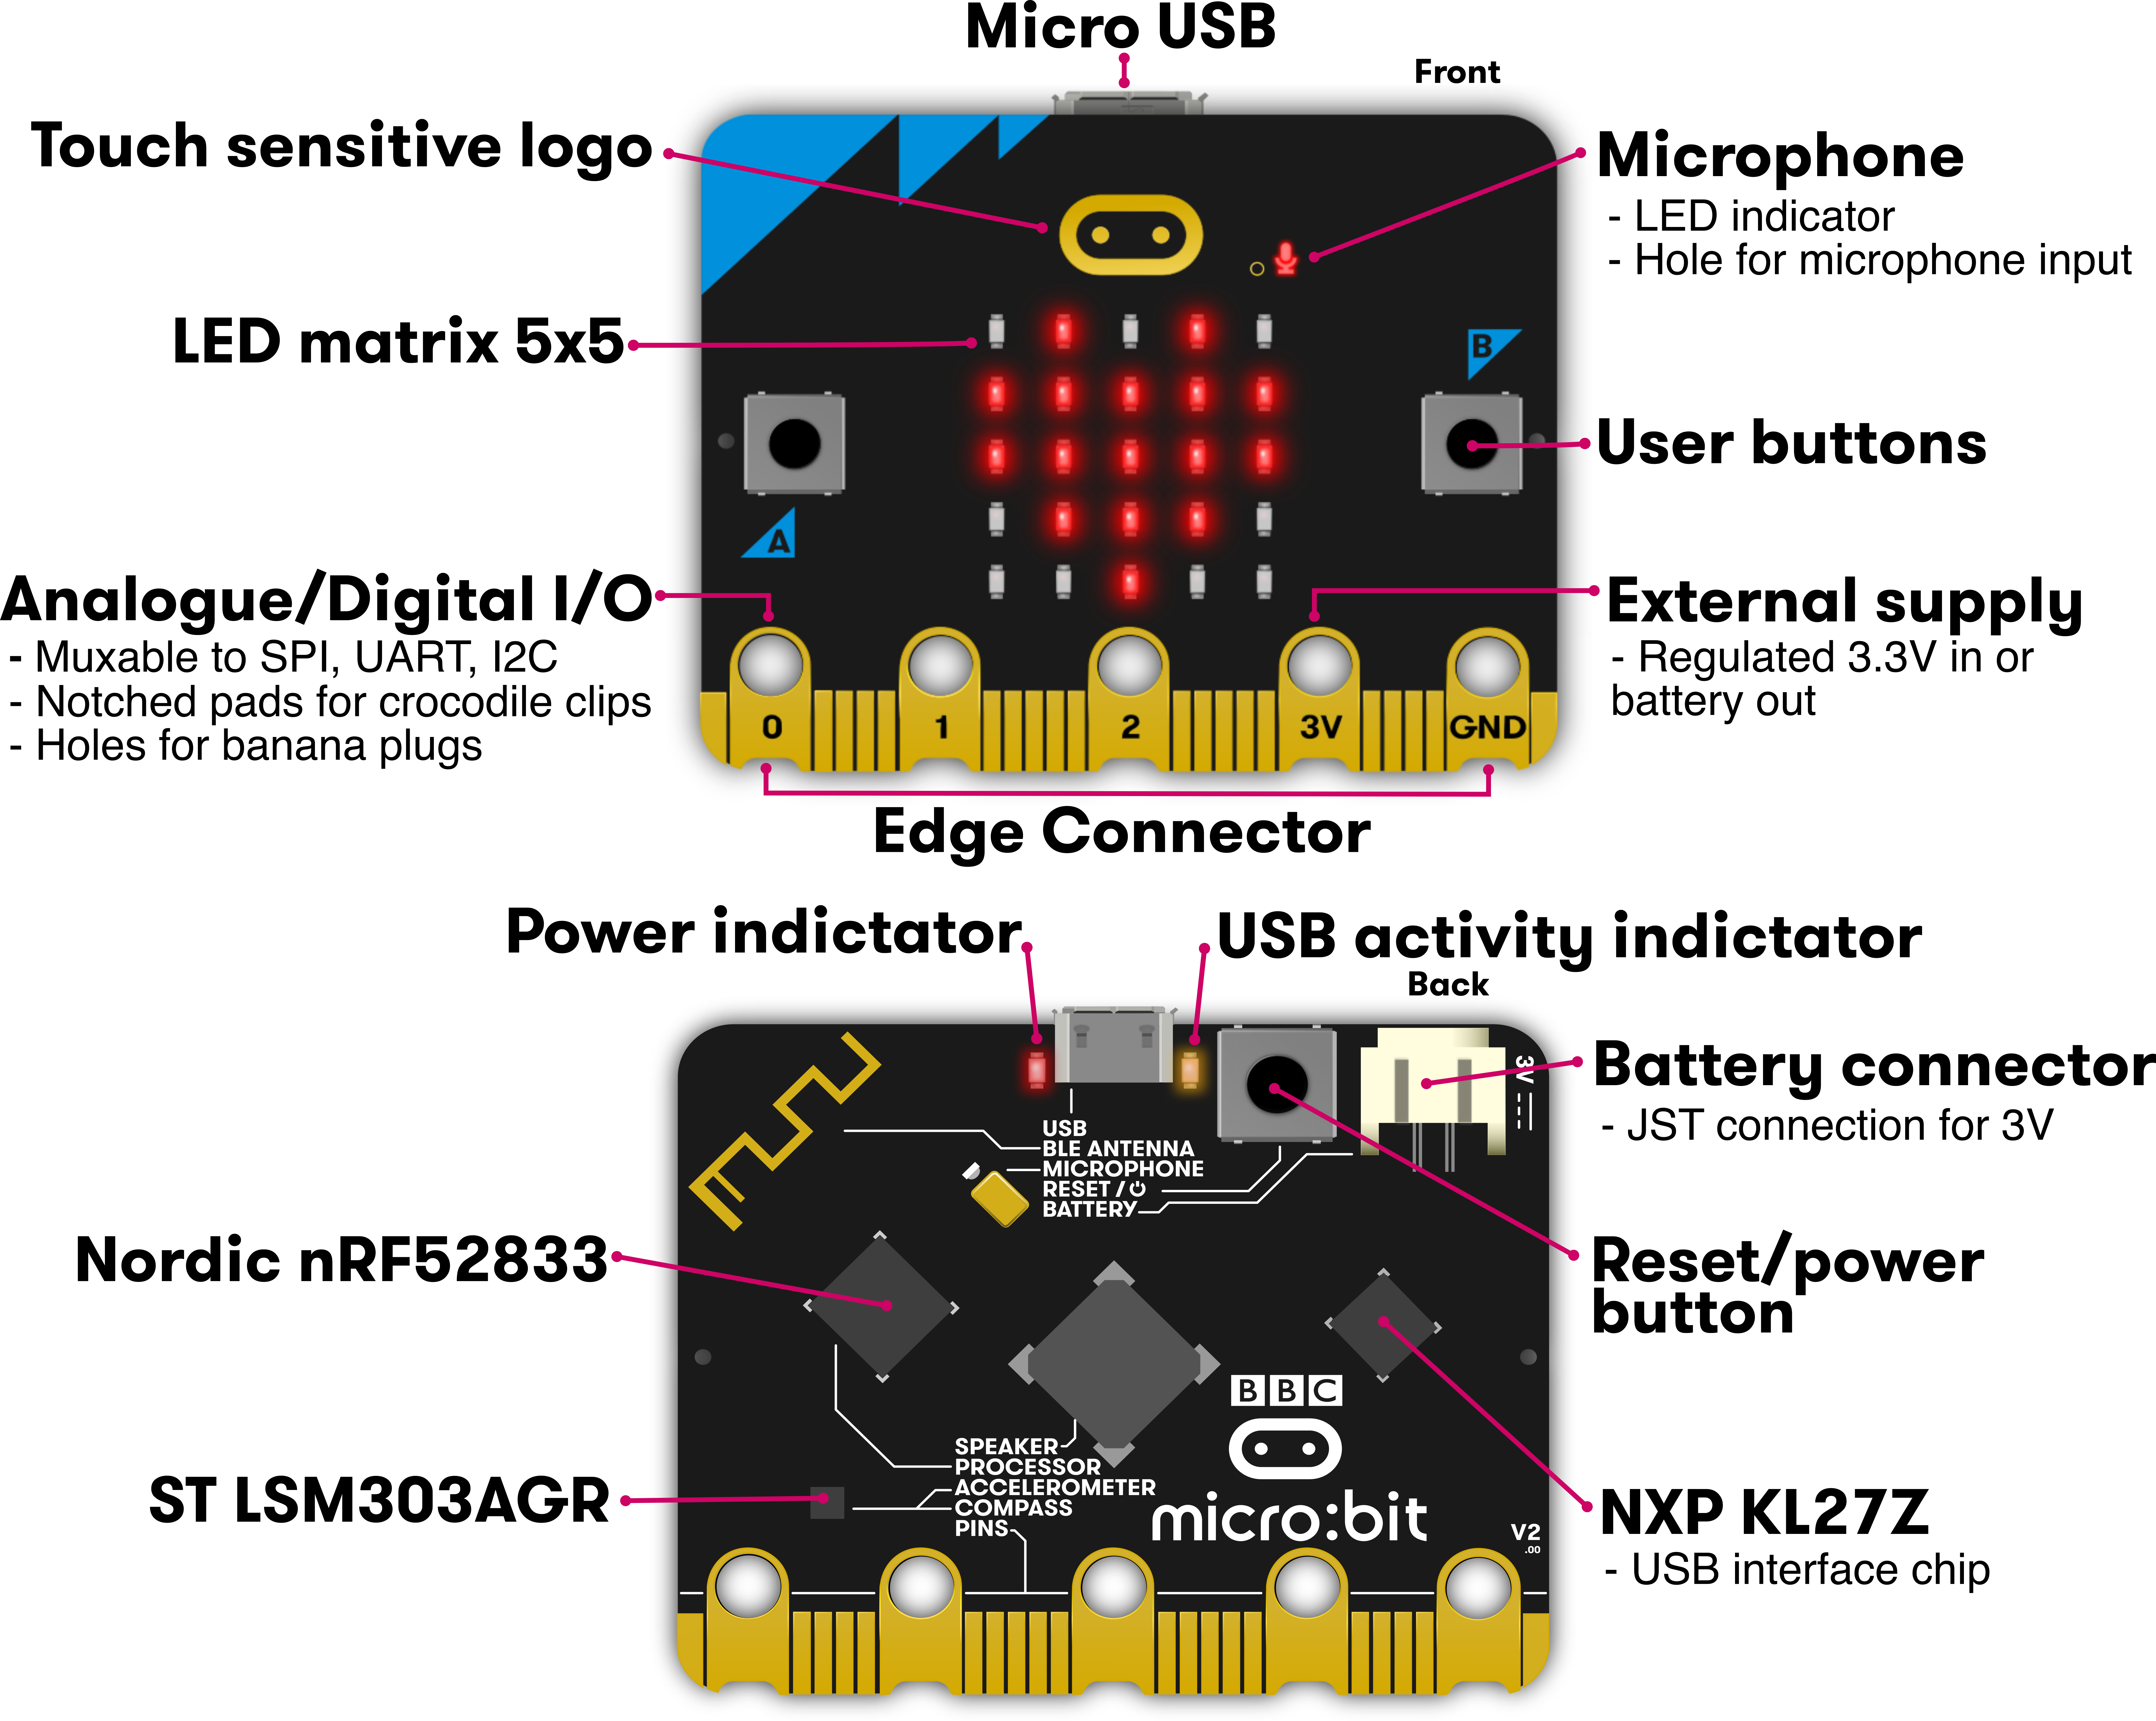
\includegraphics[width=\textwidth]{images/microbit-overview-2}
    \end{columns}    
\end{frame}

\begin{frame}{Our First Program}
    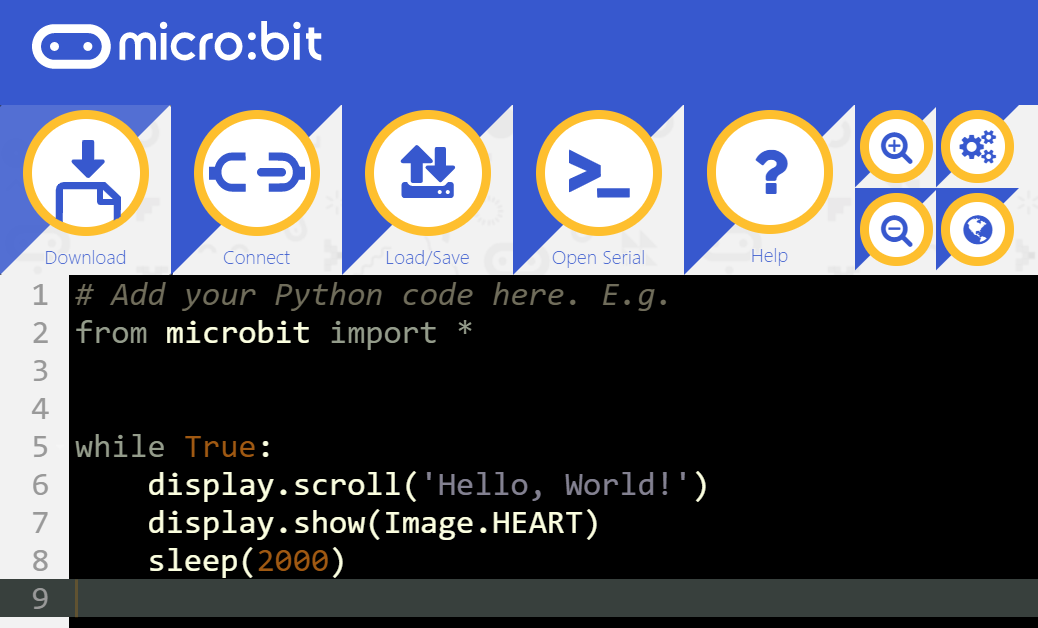
\includegraphics[max width=\textwidth, max height=\textheight]{images/prog1}
\end{frame}

\begin{frame}{Connecting}
    \begin{enumerate}
        \item Click ``Connect''
        \item Select your Micro:Bit from the menu.
        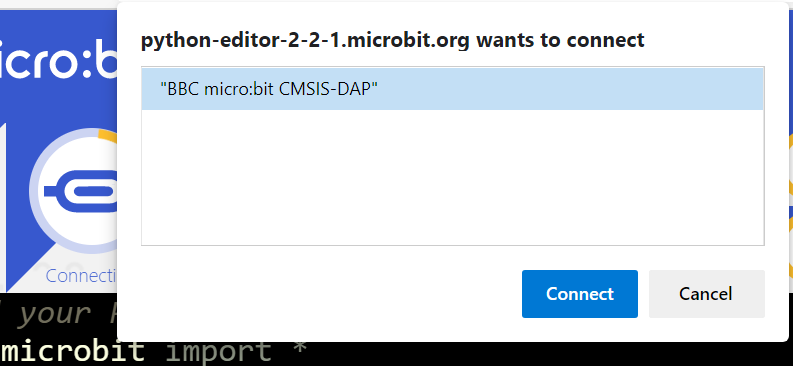
\includegraphics[max height=0.5\textheight]{images/connect}
    \end{enumerate}
\end{frame}

\begin{frame}{Flashing}
    
\includegraphics[max width=\textwidth]{images/connected-toolbar}
    \begin{enumerate}
        \item Click "Flash"
        \item Wait for flashing to complete.
    \end{enumerate}
\end{frame}

\begin{frame}{Things to Try}
    \begin{enumerate}
        \item Change the message scrolling on the screen to ``CyberCamp 2021''.
        \item Remove the line which reads \texttt{while True:}
        \item Fix the program so that it runs without that line. What effect does that line have?
        \item Let's discuss other parts of this program. What does each line do?
    \end{enumerate}
\end{frame}

\section{Working With Variables}

\begin{frame}[fragile]{A simple Numeric Variable}
    \begin{code}
# A simple program with a variable
from microbit import *


num = 0
display.show(num)
    \end{code}
\end{frame}

\begin{frame}[fragile]{Performing Arithmetic}
    \begin{code}
# Demonstrating basic arithmetic
from microbit import *


num = 0
display.show(num)
num = num + 1
display.show(num)
num = num * 3
display.show(num)
num = num - 1
display.show(num)
num = num / 2
display.show(num)
    \end{code}
\end{frame}

\begin{frame}{Things to Try}
    \begin{enumerate}
        \item Modify the arithmetic program so you can see all the results.
        \item Write a program that answers the question, ``Does python understand the order of operations?''
        \item Explore the other arithmetic operators:
        \begin{description}
            \item[\texttt{**}] Exponent
            \item[\texttt{\%}] Modulus (Remainder)
        \end{description}
    \end{enumerate}
\end{frame}

\begin{frame}[fragile]{List Variables}
    \begin{code}
# A list of micro:bit sounds
from microbit import *

sound = [Sound.GIGGLE, Sound.HAPPY, Sound.HELLO, Sound.MYSTERIOUS,
         Sound.SAD, Sound.SLIDE, Sound.SOARING, Sound.SPRING,
         Sound.TWINKLE, Sound.YAWN]

audio.play(sound[0])
sleep(1000)
audio.play(sound[9])    
    \end{code}
\end{frame}

\section{Working With Loops and Decisions}

\begin{frame}[fragile]{Play All Sounds}
    \begin{code}
# Play all the sounds!
from microbit import *

sound = [Sound.GIGGLE, Sound.HAPPY, Sound.HELLO, Sound.MYSTERIOUS,
         Sound.SAD, Sound.SLIDE, Sound.SOARING, Sound.SPRING,
         Sound.TWINKLE, Sound.YAWN]

for i in range(10):
    display.show(i)
    audio.play(sound[i])
    sleep(1000)
    \end{code}
\end{frame}

\begin{frame}[fragile]{Range}
    \begin{block}{A Closer Look}
    \begin{code}
    range(end)
    range(start, end, step)
    \end{code}
    \end{block}
    \begin{itemize}
        \item By default, starts at 0.
        \item Counts while the number is less than end.
        \item Counts by step increments.
    \end{itemize}
\end{frame}

\begin{frame}{Things to Try}
    \begin{enumerate}
        \item Play only the even numbered sounds.
        \item Test out what happens if you make the loop go too long.
    \end{enumerate}
\end{frame}

\begin{frame}[fragile]{Truth Based Loops and Decisions}
    \begin{code}
# Play all the sounds, repeatedly!
from microbit import *

sound = [Sound.GIGGLE, Sound.HAPPY, Sound.HELLO, Sound.MYSTERIOUS,
         Sound.SAD, Sound.SLIDE, Sound.SOARING, Sound.SPRING,
         Sound.TWINKLE, Sound.YAWN]

keepGoing = True

while keepGoing:
    # play the 10 sounds
    for i in range(10):
        display.show(i)
        audio.play(sound[i])
        sleep(1000)
    
    # stop if the user presses button a
    if button_a.get_presses() > 0:
        keepGoing = False
    \end{code}
\end{frame}

\begin{frame}{Something to Try}
        Modify the program so that it stops right after the current sound when you press the A button. (HINT: The \texttt{break} command will cause a loop to stop.)
\end{frame}

\begin{frame}{What is Truth?}
    \begin{itemize}
        \item Boolean Literal Values: \texttt{True}, \texttt{False}
        \item Comparisons: \texttt{==, !=, <, <=, >, >=}
        \item Boolean Operations: \texttt{and, or, not}
        \begin{table}[h]
            \centering
            \begin{tabular}{ll|lll}
                 \texttt{a} & \texttt{b} & \texttt{a and b} & \texttt{a or b} & \texttt{not a}  \\
                 \hline
                 \texttt{False} & \texttt{False} & \texttt{False} & \texttt{False} & \texttt{True}  \\
                 \texttt{False} & \texttt{True} & \texttt{False} & \texttt{True} & \texttt{True}  \\
                 \texttt{True} & \texttt{False} & \texttt{False} & \texttt{True} & \texttt{False}  \\
                 \texttt{True} & \texttt{True} & \texttt{True} & \texttt{True} & \texttt{False}  \\
            \end{tabular}
            \caption{Logical Operators}
            \label{tab:my_label}
        \end{table}
    \end{itemize}
\end{frame}


\begin{frame}[fragile]{Two Way Choices}
    \begin{code}
# Flip a virtual coin when the user presses "A"
from microbit import *
from random import *

counter = 0

while True:
    if button_a.get_presses() > 0:
        flip = random()
        if flip < 0.5:
            display.show("H")
        else:
            display.show("T")
    \end{code}
\end{frame}


\begin{frame}[fragile]{Counter}
    \begin{code}
# Count Up and Down
from microbit import *

counter = 0

while True:
    display.show(counter)
    
    #B goes up, a goes down
    if button_b.get_presses() > 0:
        counter = counter + 1
    elif button_a.get_presses() > 0:
        counter = counter - 1
    \end{code}
\end{frame}

\begin{frame}{Something to Try}
    Modify the virtual coin flip so that it is a guessing game. The game should be played this way:
    \begin{enumerate}
        \item If the user presses ``A'', they guess heads.
        \item If the user presses ``B'', they guess tails.
        \item After the user has guessed, the micro:bit will flip its virtual coin and display the result.
        \item If the guess is correct, it plays the happy sound, otherwise it plays the sad sound.
        \item After the sound, it clears the screen \texttt{display.clear()}, and the game starts over.
    \end{enumerate}
\end{frame}

\section{Animations and Games}
\begin{frame}[fragile]{Falling Flapjacks Part 1}
    \begin{code}
# Falling Flapjack
from microbit import *
from random import *

def clearLine(x, y):
    # clear the line
    display.set_pixel(x, y, 0)
    display.set_pixel(x+1, y, 0)

def drawLine(x, y):
    # clear the line
    display.set_pixel(x, y, 9)
    display.set_pixel(x+1, y, 9)
    \end{code}
\end{frame}

\begin{frame}[fragile]{Falling Flapjacks Part 1 ctd...}
    \begin{code}
flapx = [ 0, 2, 3]
flapy = [ 1, 1, 0]
flapBounceHeight = [0, 0, 0]
flapDirection = [1, 1, 1]


while True:
    # update the flapjacks
    for i in range(3):
        # move the flapjack
        clearLine(flapx[i], flapy[i])
        flapy[i] += flapDirection[i]
        drawLine(flapx[i], flapy[i])
        
        
        # handle bouncing off the bottom
        if flapy[i] == 4:
            flapBounceHeight[i] = randint(0, 2)
            flapDirection[i] = -1

        # handle reaching maximum bounce height
        if flapy[i] == flapBounceHeight[i]:
            flapDirection[i] = 1
    
    # 2 frames per second!
    sleep(500)
    \end{code}
\end{frame}


\begin{frame}{Challenge 1 - Add A Player Paddle}
    Add a player paddle on row 4 (the bottom.) 
    \begin{itemize}
        \item Button A moves left and Button B moves right.
        \item Make sure the paddle does not move off the screen!
    \end{itemize}
\end{frame}


\begin{frame}{Challenge 2 - Bounce ONLY off the Paddle}
    Alter the code so that the flapjacks only bounce of the paddle.
    \begin{itemize}
        \item If the player hits the flapjack, it bounces to a random height.
        \item If the player misses a flapjack, the game ends.
    \end{itemize}
\end{frame}


\begin{frame}[fragile]{Challenge 3 - Add Sound Effects}
    Add sound effects for bounces and game over.
    \begin{block}{Hint}
    You can play a sound without waiting for it complete. For example:
    \begin{code}
    audio.play(Sound.Twinkle, wait=False)
    \end{code}
    \end{block}
\end{frame}

\end{document}
